% --- chapter
\newcommand{\chapter}[2][]{
	\newcommand{\chapname}{#2}
	\begin{flushleft}
		\begin{minipage}[t]{\linewidth}
			
\includegraphics[height=1cm]{hdht-logo.png}
			\hspace{0pt}	
			\sffamily\bfseries\large Bài  24. Tán sắc ánh sáng
			\begin{flushleft}
				\huge\bfseries #1
			\end{flushleft}
		\end{minipage}
	\end{flushleft}
	\vspace{1cm}
	\normalfont\normalsize
}
%-----------------------------------------------------
\chapter[Tán sắc ánh sáng]{Tán sắc ánh sáng}

\section{Lý thuyết}

\subsection{Nguyên nhân của hiện tượng tán sắc}
\begin{itemize}
	\item Chiết suất tuyệt đối của môi trường trong suốt: 
	\begin{equation}\label{eq:tansac1}
		n=\dfrac{c}{v}= \dfrac{cT}{vT}=\dfrac{\lambda}{\lambda'},
	\end{equation}
	trong đó, $\lambda$ và  $\lambda'$ là bước sóng ánh sáng trong chân không và trong môi trường trong suốt cần tính, $c$ và $v$ là vận tốc ánh sáng trong chân không và trong môi trường đó.
	
	\item Nguyên nhân của hiện tượng tán sắc là đo chiết suất của môi trường trong suốt phụ thuộc màu sắc của ánh sáng và tăng dần từ màu đỏ đến màu tím 
		\begin{equation}\label{eq:tansac2}
	n_\text{đỏ} < n_\text{cam} <n_\text{vàng} < n_\text{lục} <n_\text{lam} < n_\text{chàm} < n_\text{tím}.
		\end{equation}
	\item Hiện tượng tán sắc chỉ xảy ra khi chùm sáng phức tạp (gồm nhiều bước sóng khác nhau) bị khúc xạ qua mặt phân cách hai môi trường trong suốt.
	\item Tia đỏ lệch ít nhất (góc lệch nhỏ nhất, góc khúc xạ lớn nhất) và tia tím lệch nhiều nhất (góc lệch lớn nhất, góc khúc xạ nhỏ nhất).
\end{itemize}
\luuy{Khi sóng truyền từ môi trường từ môi trường này sang môi trường khác
	\begin{itemize}
		\item tần số \textit{không thay đổi}.
		\item vận tốc truyền và bước sóng \textit{thay đổi}
	\end{itemize}
	}
	
\subsection{Tán sắc ánh sáng qua lăng kính}
\begin{center}
	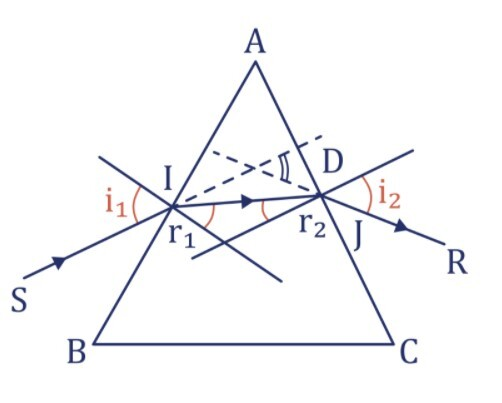
\includegraphics[scale=0.5]{../figs/VN12-PH-32-A-016-1-2.jpg}
\end{center}
Công thức của lăng kính
	\begin{equation}\label{eq:tansac3}
		\begin{array}{rcl}
			\sin i_1&=&n\sin r_1\\
				\sin i_2&=&n\sin r_2\\
				A&=&r_1+r_2\\
				D&=&i_1+i_2-A
		\end{array}
	\end{equation}
\luuy{
	Nếu các góc nhỏ hơn $10^\circ$ thì công thức gần đúng của lăng kính là:
	\begin{equation}\label{eq:tansac4}
	\begin{array}{rcl}
	i_1&=&n r_1\\
	i_2&=&n r_2\\
	A&=&r_1+r_2\\
	D&=&(n-1)A
	\end{array}
	\end{equation}
 }

\section{Mục tiêu bài học - Ví dụ minh họa}

\begin{dang}{Nguyên nhân của hiện tượng tán sắc.}
\ppgiai{
\begin{description}
\item [Bước 1] Áp dụng công thức $ n=\dfrac{c}{v}= \dfrac{cT}{vT}=\dfrac{\lambda}{\lambda'} $ để xác định chiết suất tuyệt đối, bước sóng, tần số. 
\item [Bước 2] Áp dụng công thức $ n_\text{đỏ} < n_\text{cam} <n_\text{vàng} < n_\text{lục} <n_\text{lam} < n_\text{chàm} < n_\text{tím} $ để so sánh và biện luận chiết suất môi trường với những ánh sáng khác nhau 
\end{description}
}

\viduii{2}{Bước sóng trong chân không của ánh sáng đỏ là \SI{0.75}{\micro\meter}. Tính bước sóng của các ánh sáng đó trong thuỷ tinh, biết chiết suất của thuỷ tinh đối với tia đỏ là 1,5 và đối với tia tím là 1,54.
	}
	{	
		\begin{center}
			\textbf{Hướng dẫn giải}
		\end{center}
		
		Bước sóng ánh sáng trong môi trường $\lambda ' =\dfrac{\lambda}{n}$ (với $n$ là chiết suất tuyệt đối của môi trường).
		
		\begin{itemize}
			\item Bước sóng của ánh sáng đỏ trong thủy tinh
			
			\begin{equation*}
			\lambda'_{\text{đ}} =\dfrac{\lambda_{\text{đ}}}{n}=\dfrac{\text{0,75}}{\text{1,5}}=\text{0,5}\ \mu \text{m}.
			\end{equation*}
			\item Bước sóng của ánh sáng tím trong thủy tinh
			
			\begin{equation*}
			\lambda'_{\text{t}} =\dfrac{\lambda_{\text{t}}}{n}=\dfrac{\text{0,4}}{\text{1,54}}\approx \text{0,26}\ \mu \text{m}.
			\end{equation*}
		\end{itemize}
		
	\begin{center}
	\textbf{Câu hỏi tương tự}
	\end{center}

	Bước sóng của ánh sáng đỏ trong không khí là $ \SI{0.64}{\mu m} $. Tính 	bước sóng của ánh sáng đỏ trong nước biết chiết suất của nước đối với ánh sáng đỏ là $ \dfrac{4}{3} $.
	\begin{mcq}(4)
		\item \SI{0,24}{\mu m}.
		\item \SI{0,48}{\mu m}.
		\item \SI{0,36}{\mu m}.
		\item \SI{0,54}{\mu m}.
	\end{mcq}
	\textbf{Đáp án:} B.
	}
	
\viduii{2}{
	Một bức xạ đơn sắc có tần số $4\cdot 10^{14}\ \text{Hz}$. Biết chiết suất của thuỷ tinh đối với bức xạ trên là 1,5 và tốc độ ánh sáng trong chân không bằng $3\cdot 10^8\ \text{m/s}$. Bước sóng của nó trong thuỷ tinh là
			\begin{mcq}(4)
				\item \SI{0.64}{\micro\meter}	
				\item \SI{0.5}{\micro\meter}
				\item \SI{0.55}{\micro\meter}
				\item \SI{0.75}{\micro\meter}	
			\end{mcq}
	}
	{	\begin{center}
			\textbf{Hướng dẫn giải}
		\end{center}
		
		\begin{itemize}
	\item Bước sóng của ánh sáng trong chân không
	\begin{equation*}
		\lambda =\dfrac{c}{f}=\dfrac{3\cdot 10^8}{4\cdot 10^{14}}=\text{7,5}\cdot 10^{-7}\ \text{m}.
	\end{equation*}
	\item Bước sóng của ánh sáng trong thủy tinh
	\begin{equation*}
		\lambda' =\dfrac{\lambda}{n}=\dfrac{\text{7,5}\cdot 10^{-7}}{\text{1,5}}= 5 \cdot 10^{-7}\ \text{m}.
	\end{equation*}
\end{itemize}
		
	\begin{center}
	\textbf{Câu hỏi tương tự}
	\end{center}

Biết tốc độ của ánh sáng trong chân không là $ \SI{3e8}{m/s} $. Nếu ánh sáng đơn sắc có tần số $ \SI{6 e14}{Hz} $ thì có bước sóng bằng
\begin{mcq}(4)
	\item $ \SI{0,5}{\mu m} $.
	\item $ \SI{0,5}{mm} $.
	\item $ \SI{0,5}{nm} $.
	\item $ \SI{0,5}{pm} $.
\end{mcq}
	
	
	\textbf{Đáp án:} A.
	}
\end{dang}

\begin{dang}{Tán sắc ánh sáng qua lăng kính.}
\ppgiai{
\begin{description}
\item[Bước 1] Xác định các dữ kiện đề bài cho là góc chiết quang, chiết suất, hay góc tới hoặc góc lệch. 
\item[Bước 2] Lựa chọn các công thức trong hệ \eqref{eq:tansac3} hoặc \eqref{eq:tansac4} để lần lượt tìm các đại lượng cần. 
\end{description}
}

\viduii{2}{Lăng kính có góc chiết quang $A=30^\circ$, chiết suất $n=\text{1,5}$. Chiếu vào mặt bên của lăng kính một tia sáng có góc tới $i=40^\circ$. Góc lệch của tia sáng qua lăng kính gần bằng
\begin{mcq}(4)
	\item $15^\circ$
	\item $17^\circ$.
	\item $19^\circ$.
	\item $21^\circ$.
\end{mcq}
	}
	{	\begin{center}
			\textbf{Hướng dẫn giải}
		\end{center}
		
	Áp dụng công thức:
\begin{equation*}
	\sin i_1=n\sin r_1.
\end{equation*}

Với $i_1=40^\circ,\ n=\text{1,5} $. Ta tìm được $r_1=\text{25,37}^\circ$.

Áp dụng công thức:
\begin{equation*}
	A=r_1+r_2.
\end{equation*}

Với $r_1=\text{25,37}^\circ,\ A=30^\circ$. Ta tìm được $r_2=\text{4,62}^\circ$.

Áp dụng công thức

\begin{equation*}
	\sin i_2=n\sin r_2.
\end{equation*}

Với $r_2=\text{4,62}^\circ,\ n=\text{1,5} $. Ta tìm được $i_2\approx \text{17}^\circ$.

Góc lệch của tia sáng qua lăng kính gần bằng $\text{17}^\circ$.
		
	\begin{center}
	\textbf{Câu hỏi tương tự}
	\end{center}

Một lăng kính có góc chiết quang $ A = 30\circ $. Một tia sáng đơn sắc tới mặt bên lăng kính dưới góc tới $ i_{1} = 30\circ $. Biết $ r_{1} = r_{2} $. Góc lệch $ D $ của tia sáng truyền qua lăng kính là
\begin{mcq}(4)
	\item $ 20 \circ $.
	\item $ 10 \circ $.
	\item $ 30 \circ $.
	\item $ 40 \circ $.
\end{mcq}
	
	\textbf{Đáp án:} C.
	}
	
\viduii{2}{Một lăng kính có tiết diện thẳng là tam giác ABC góc A bằng $60^\circ$ đặt trong không khí. Một chùm tia sáng đơn sắc màu lam hẹp song song đến mặt AB theo phương vuông góc cho tia ló đi là trên mặt AC. Tính chiết suất của chất làm lăng kính đối với màu lam. Thay chùm tia màu lam bằng chùm tia sáng trắng gồm 5 màu cơ bản đỏ, vàng, lục, lam, tím thì các tia ló ra khỏi mặc AC gồm những màu nào?

	}
	{	\begin{center}
			\textbf{Hướng dẫn giải}
		\end{center}
		
	\begin{itemize}
\item Chiết suất của chất làm lăng kính đối với màu lam
\begin{equation*}
	1 \cdot \sin 90^\circ = n_{\text{lam}} \cdot \sin 60^\circ \Rightarrow n_{\text{lam}}=\text{1,15}.
\end{equation*}
\item Công thức tính góc giới hạn để xảy ra hiện tượng phản xạ toàn phần
\begin{equation*}
	\sin i_{\text{gh}}=\dfrac{1}{n}.
\end{equation*}
\item Chiết suất đối với ánh sáng tím sẽ lớn hơn chiết suất đối với ánh sáng lam nên 
 \begin{equation*}
 	\dfrac{1}{n_{\text{lam}}}>\dfrac{1}{n_{\text{tím}}},
 \end{equation*}
\end{itemize}

nên chỉ có tia tím bị phản xạ toàn phần.

Suy ra tia ló khỏi lăng kính gồm đỏ, vàng, lục.
		
	\begin{center}
	\textbf{Câu hỏi tương tự}
	\end{center}

Một lăng kính có tiết diện thẳng là tam giác ABC góc A bằng $60^\circ$ đặt trong không khí. Một chùm tia sáng đơn sắc màu lục hẹp song song đến mặt AB theo phương vuông góc cho tia ló đi là trên mặt AC. Tính chiết suất của chất làm lăng kính đối với màu lam. Thay chùm tia màu lam bằng chùm tia sáng trắng gồm 5 màu cơ bản đỏ, vàng, lục, lam, tím thì các tia không ló ra khỏi mặc AC gồm những màu nào? \\

	\textbf{Đáp án:} Tia màu lam và màu tím không ló ra khỏi lăng kính.
	}
\end{dang}